\documentclass{article}
\usepackage[margin=.5in]{geometry}
%\usepackage[utf8]{inputenc}
\usepackage{multicol}
\usepackage[boxruled,vlined]{algorithm2e}
\usepackage{verbatim}
\usepackage{hyperref}
\usepackage{graphicx}
\usepackage{float}
\usepackage{subcaption}
\usepackage{amsmath}
\usepackage{amssymb}
\usepackage{amsfonts}

\graphicspath{{ ./ }}

\title{Killing Zombies in Minecraft With Deep Reinforcement Learning}
\author{Hiroto Udagawa, Tarun Narasimhan, Shim-Young Lee}
\date{December 16, 2016}

\begin{document}
\maketitle

\begin{multicols}{2}

\section{Introduction}

In this project, we train an agent in the video game Minecraft with reinforcement learning to kill as many zombies as possible in a confined space. Our agent is only equipped with a sword to attack the zombies,  which can themselves attack and kill the agent.
The objective is to have the agent learn what policies to execute based on the visual information it receives about the surroundings from the raw pixels of the game play screen and the reward structure we have designed.
Using a convolutional neural network and Q-function reinforcement learning, the agent showed definite improvement in its ability to kill zombies.
This project displays the promise of combining deep learning with reinforcement learning to achieve non-trivial tasks.






\section{Related Work}

There have been several projects in this area which we drew upon for our project.
The major inspiration for our work was DeepMind's 2013 paper on deep reinforcement learning, in which the agent was trained with a single model architecture (Deep Q Learning) that uses a convolutional neural network to perform a variant of Q-learning, and successfully played 7 different Atari 2600 games, in a few of which the agent outperformed human experts \cite{deepMind}.
Instead of solving the standard action-value function (Q function) with Bellman equations, deep convolutional neural network was used as a nonlinear function approximator. DeepMind also employed a biology inspired technique known as experience replay, which attempts to fix the divergence due to correlation between sequential inputs.
While a different network was trained for each game, the same architecture and hyperparameters were used across all of the games.
Furthermore, no prior (or game specific) knowledge was used, but only the raw pixel values were fed to the network as inputs.
DeepMind's major achievement was using extremely high-dimensional states (the visual input from the agent) and no information about the game rules to train an algorithm which could outperform skilled human players, and we aimed to replicate this in our project.

For the actual implementation of our project, we built on the work of Chen (2015), which also relied on DeepMind's DQN and applied the same model architecture and algorithm to the game Flappy Bird \cite{flappyBird}.
We sought to expand on his work by applying DeepMind's architecture to a more complicated setting.
While Flappy Bird has only two possible actions and no opponents, Minecraft has a continuous action space and our setting includes zombies actively trying to kill the agent.




\section{Minecraft and Project Malmo}

For the setting of our project, we chose Minecraft, a popular sandbox video game that was released in 2011. It allows players to control an agent, through which they can explore the map, build structures, craft tools, and destroy computer-generated zombies.
Project Malmo is an open source platform for Minecraft created by Microsoft that offers an interface for researchers to experiment with different approaches to artificial intelligence by controlling an agent through Python scripts.

Malmo is a useful environment for artificial intelligence research because it allows users to test endless situations within a relatively simple framework by  controlling agents' movements and environments via code.
By combining different states, actions, and spaces, researchers can create different environments and define various tasks for which the agent trains with reinforcement learning.

As a simulator, Malmo is more constrained than many other simulators which researchers have employed. Microsoft designed Malmo to be an interface with Minecraft, but not to provide the agent with any information about Minecraft.
Thus, the default in Malmo is for the player-controlled agent to not have any information about its environment or the rules of the game.
This feature makes Malmo very convenient for reinforcement learning as this replicates the exact kind of environment we want for reinforcement learning: in order to maximize difficulty, the agent should be trained only from its own visual input.
For example, the agent does not "know" that the \emph{attack} action kills zombies; it learns this through training.

An additional constraint posed by Minecraft is the fact that the field of view is first person.
In many or the Atari games tested by DeepMind or in Flappy Bird, the game gives a bird's-eye view, which gives much more information than the agent's first-person view in Minecraft.
For example,
[{\bf Hiro: do you want to discuss Minecraft/Malmo implementation issues here? Like the lag issue?}]




\section{Method}



\subsection{Scenario}

The agent begins in the middle of a completely flat room with a fixed number of randomly generated zombies. The room has a uniform color so that the algorithm will not have to account for differences in lighting and colors. The zombies automatically approach the agent and damage it if they get too close. The agent will be equipped with a sword to fend off the zombies. As the agent destroys zombies, new zombies continue to spawn (so that there is always a constant number of zombies), and the game continues to run until the character loses all of its health. At this time, the score will be calculated based on the total number of zombies that the character was able to kill and the scenario resets to the beginning.

\begin{figure}[H]
\caption{Minecraft screenshot}
\centering
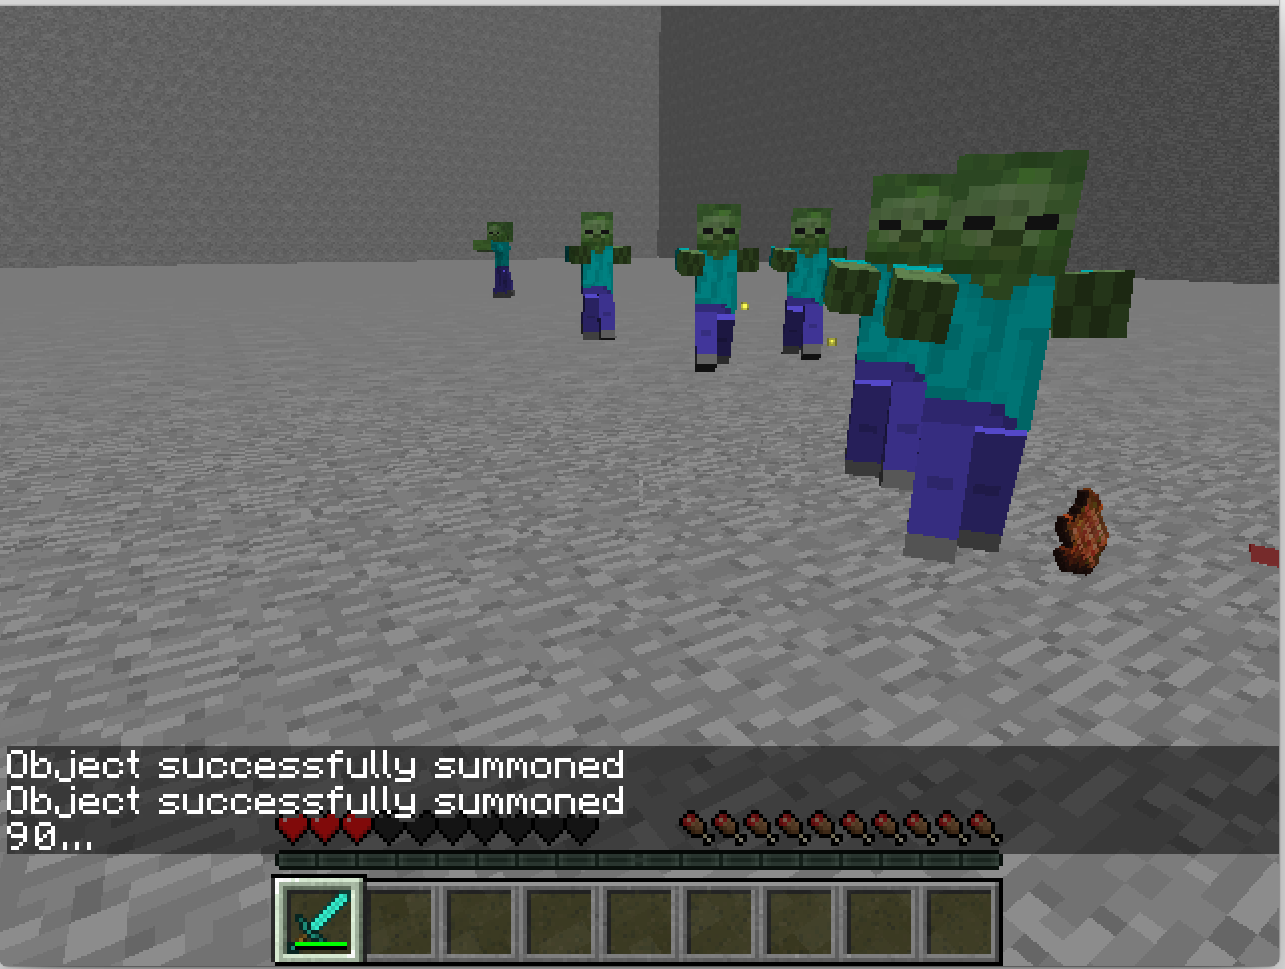
\includegraphics[scale=0.3]{./hiro_screenshot.png}
\end{figure}

\subsection{MDP Formulation}

We formalize the reinforcement learning task with Markov Decision Process.
The agent interacts with an environment by making observations and actions, and receiving rewards.
At each iteration, the agent selects an action from the action space, $A = {1, . . . , K }$.
Agent's action in turn changes the state the agent is in and the agent receives rewards based on the new state it enters.
The reward often depends not only on the new state it just entered, but the entire sequence of actions and observations it made until it entered the current state.
Thus, to make an appropriate action in the current state, the agent needs information from previous actions and observations as well as the current observation. We therefore consider sequences of actions and observations $s_t = x_1, a_1, x_2, ..., a_{t-1}, x_t$. All such sequences are finite; thus we now have finite Markov decision process (MDP), where we use the sequence $s_t$ as a distinct state at each time-step $t$.

\subsubsection{Actions and States}

The actions for this problem are the discrete movements of the agent (the agent can move forward, back, turn left, turn right, or remain stationary) as well as the ability to attack with a sword. To simplify the action space, the attack command was turned on the entire time, and the agent only chooses how to move at each time-step. Minecraft allows the agent to move and turn with different speed, but we only use five possible actions with fixed moving and turning speed.

The observation at time-step $t$, $x_t$, is an image of the player's vision represented by the pixels values.
Project Malmo provides the functionality to retrieve the image from the screen.
As stated earlier, the state at time-step $t$ is a sequence of observations and actions made until and at time $t$.


\subsubsection{Reward}

We assign the algorithm a reward of +1 for a successful hit on a zombie and a reward of +5 for a successful kill.
There is also a reward of 0.03 for every frame for which it stays alive and a penalty of -1 for every time the agent gets hit. These are designed to train the agent's behavior to incentivize staying alive; holding the kill count equal, we wanted the agent to have a higher reward for staying alive longer.


\subsection{Q-learning and Deep Q Network}

\subsubsection{Reinforcement Learning Background}

In reinforcement learning, the agent is to trained to maximize aggregate future rewards. With the discount factor of $\gamma$, the future discounted return at time $t$ is $R_t = \sum_{t' = t}^T \gamma^{t' - t}r_{t'}$, where $T$ is the number of time-steps (or iterations) in that episode of the game.
We define the optimal action-value function
$Q^{*}(s, a) = \max_\pi \mathbb{E}[R_t | s_t = s, a_t = a, \pi]$,
which is the maximum expected return achievable by following any strategy,
after seeing some sequence $s$ and then taking some action $a$, and where $\pi$ is a policy mapping sequences to actions (or distributions over actions).

In simpler settings, the optimal policy is obtained by solving the Bellman equation iteratively, using the equation $Q_i^*(s,a) = \mathbb{E}[r +  \max_{a'} Q^* (s', a' )| s, a]$.
However, maintaining estimates of action-value function for all sequences (states) is impossible and yields no generalization for newly encountered states.
This is especially problematic in our setting, where the number of states is extremely large due to the high dimensionality of our input (i.e. pixels from the agent's visual input).

Instead, we use a convolutional neural network as a nonlinear function approximator to estimate the action-value function. We train the neural network approximator $Q(s,a,\theta)$ by minimizing a loss functions $L_i(\theta)$ defined for each iteration $i$, (where $\theta$ are the Q-network weights)

\begin{equation*}
    L_i(\theta_i) = \mathbb{E}_{s,a \sim \rho(·)} [(y_i - Q (s, a; \theta_i))^2]
\end{equation*}


where $y_i = \mathbb{E}_{s' \sim \epsilon}[r + \gamma \max_{a'} Q(s', a'; \theta_{i-1} | s, a]$ is the target for iteration $i$ and $\rho(s, a)$, the behaviour distribution, is a distribution over states $s$ and actions $a$.
Note that the target value used in iteration $i$ is calculated with the previous iteration's network weights. For faster computation at each iteration, stochastic gradient descent is used; instead of calculating the expectation, we update the weights with a single sample from distribution.

\subsubsection{Deep Q Network}

Since the observation the agent receives is an image (pixel values) of the gameplay screen, convolutional neural network is a reasonable choice of neural network. Although in the formulation of the MDP we stated that each state is an entire sequence of actions and observations, neural networks can only handle fixed input size. Furthermore, the state(sequence) contains actions as well as images, but including action in the input layer requires multiple forward passes, getting the actiona-value funciton output for each action in the action space. To deal with these issues, we 1) only use the 3 most recent images instead of the entire sequence, and 2) use a network architecture in which only the image is fed to the input layer and outputs are estimates of Q value for each possible action. For the detailed explanation of the exact network architecture, see section 'Training'. 

We instead use an architecture in which there is a separate output unit for each possible action, and only the state representation is an input to the neural network. The outputs cor- respond to the predicted Q-values of the individual actions for the input state. The main advantage of this type of architecture is the ability to compute Q-values for all possible actions in a given state with only a single forward pass through the network.

\subsubsection{Experience Replay}

Often, there is a delay between actions and resulting rewards, and little association between the most recent input and the reward it just received. Also, the inputs are not independent, since the subsequent(consecutive?) inputs are highly correlated. Furthermore, the distribution of the input states is influenced heavily by recently taken actions will vary widely if we use only the recently obtained frames as inputs.    

These issues can lead to neural network taking too long to converge, or being very unstable and unable to learn efficiently. To de-correlate the inputs and stabilize the fluctuation of input sampling distribution, we use the technique named experience replay. During gameplay keep a fixed number of most recent experiences {s, a, r, s'} in a replay memory, and train the network with random batches of experiences(states/sequences) sampled from the memory, rather than the most recently obtained states. 

\subsubsection{$\epsilon$-greedy policy}

 e-greedy strategy that follows the greedy strategy with probability 1-e and selects a random action with probability e.


\subsection{Training}

\subsubsection{Preprocessing}

The raw pixel frames we can get through Malmo platform is 480 x 640 x 3 with 256 possible values for each color channel. To reduce the input to more manageable size, the images were preprocessed: we converted the image from the RGB to grayscale and rescaled it to 84 x 84. Since the actual input fed into the neural network is a stack of 3 most recent frames, the final input dimension is 84 x 84 x 3. 

\subsubsection{Model Architecture}

The overall neural network consists of three convolutional layers and two fully connected layers. The input layer takes an 84 x 84 x 3 preprocessed image. The first hidden layer convolves the input with 32 filters of 8 x 8 with stride 4 and applies a rectifier nonlinearity. The second hidden layer convolves with 64 filters of 4 x 4 with stride 2, followed by a rectifier nonlinearity. The third layer convolves 64 filters of 3 x 3 with stride 1, again followed by a rectifier. The final hidden layer is fully-connected layer of 512 rectifier units. The output layer is a fully-connected linear layer (no rectifier) with an output node for each action in the action space. Our network has 5 output nodes. The following table summarizes the input and filter size at each layer of the network.

\begin{tabular}{|l|l|l|l|l|l|}
        \hline
Layer & Input    & Filter size & Stride & Num Filters & Output   \\ \hline
conv1 & 84x84x3  & 8x8         & 4      & 32          & 20x20x32 \\ \hline
conv2 & 20x20x32 & 4x4         & 2      & 64          & 9x9x64   \\ \hline
conv3 & 9x9x64   & 3x3         & 1      & 64          & 7x7x64   \\ \hline
fc4   & 7x7x64   &             &        & 512         & 512      \\ \hline
fc5   & 512      &             &        & 18          & 18     \\ \hline
\end{tabular}
  
\subsubsection{Algorithm}

We use Q-learning to have our agent learn a policy to best fight these zombies.
We utilize the work done by Google Deep Mind to use a convolutional neural network to approximate the Q-function iteration after iteration.
\paragraph{}


\begin{algorithm*}[H]
     \SetAlgoLined
     initialize Q function with random weights \;
     observe initial state $S$ \;
     \Repeat{terminated} {
        with probability $\epsilon$ generate random action \;
        otherwise select $a = \arg\max_{a'} Q(s,a')$ \;
        carry out action $a$ \;
        observe reward $r$ and new state $s'$ \;
        update $D$ with new data: $<s,a,r,s'>$ \;
        sample random transitions from $D$ \;
        update network \;
     }
     \caption{Adapted from Mnih et al, 2015}
\end{algorithm*}

\begin{figure}[H]
\caption{Images of processed features}
\begin{subfigure}{.25\textwidth}
  \centering
  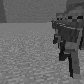
\includegraphics[scale=1.0]{./messigray1.png}
  \caption{1a}
  \label{fig:sfig1}
\end{subfigure}%
\begin{subfigure}{.25\textwidth}
  \centering
  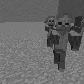
\includegraphics[scale=1.0]{./messigray2.png}
  \caption{1b}
  \label{fig:sfig2}
\end{subfigure}
%\vskip\baselineskip
\begin{subfigure}{.25\textwidth}
  \centering
  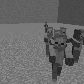
\includegraphics[scale=1.0]{./messigray3.png}
  \caption{1c}
  \label{fig:sfig3}
\end{subfigure}
\label{fig:fig}
\end{figure}



\section{Results and Analysis}

The agent kicks ass and takes names like Chuck Norris on cocaine.

\begin{description}
    \item[Table 1: Learning rate under varying Reward Structures]
    \item[Table 2: Learning rate under varying $\epsilon$]
    \item[Table 3: Learning rate under varying learning rates]
    \item[Table 4: Learning rate under varying difficulties]
\end{description}

We ran into the unexpected problem that...





\section{Conclusions and Future work}
We succesfully trained a Deep Q Network to move around a room and kill zombies by taking visual input from the agent.
Our results suggest that \emph{foo} and \emph{bar} methods worked best because [...]

Future work on this task might focus on expanding the agent's action space so that the agent can execute continuous movements rather than the discretized actions we have programmed.
Additionally, researchers could focus on improving DeepMind's convolutional neural network to further enhance the performance or learning curve of the algorithm.
This might involve different gradient algorithms or initial weights.

\end{multicols}





%%%%%%%%%%%%%%%%%%%%%%%%%%%%%%%%%%%%%%%%%%%%%%%%%%%%
%%%%%%%%%%%%%%%%%%% Bibliography %%%%%%%%%%%%%%%%%%%
%%%%%%%%%%%%%%%%%%%%%%%%%%%%%%%%%%%%%%%%%%%%%%%%%%%%
\pagebreak
\begin{thebibliography}{9}


\bibitem{deepMind}
Mnih, Volodymyr; Kavukcuoglu, Koray; Silver, David; Graves, Alex; Antonoglou, Ioannis; Wierstra, Daan; Riedmiller, Martin.
\emph{Playing Atari with Deep Reinforcement Learning},
December 2013.

\bibitem{nervanasys}
Matiisen, Tambet.
\emph{Demystifying Deep Reinforcement Learning}. December 2015.
\url{https://www.nervanasys.com/demystifying-deep-reinforcement-learning/}

\bibitem{flappyBird}
Chen, Kevin.
\emph{Deep Reinforcment Learning for Flappy Bird}


\end{thebibliography}


\end{document}
